\chapter{The Large Hadron Collider} \label{chap:lhc}

Located 100 meters under the Swiss / French boarder lies the 26.7 kilometer
Large Hadron Collider (LHC) \cite{Evans:2008zzb}.  The culmination of a huge international collaboration,
this apparatus is used to produce proton and heavy ion collisions for observation by
the four major experiments at the LHC: ATLAS, CMS, LHCb, and ALICE.  The system
was designed for a maximum center-of-mass  energy of $\sqrt{s} = 14$ TeV and a peak
instantaneous luminosity of $L = 10^{34} $cm$^{-2} $s$^{-1}$.  

The first LHC workshop was held in 1984 in Lausanne at the European Organization
for  Nuclear Reserach (CERN).  The nearly 30 year old case for a machine that 
would push towards the discovery of the elusive Higgs Boson was presented using
the existing CERN accerlerator facilities and the Large Electron Positron (LEP)
collider tunnel. The proposal became reality on September 10, 2008 when the
first proton beams were circulated, only to have calamity strike 9 days later in
the form of a catastrophic electrical fault. The repairs and improvements lasted
until November 2009 when the LHC restarted.  Since then this modern marvel has
worked wonderfuly and, as hoped, lead to the discovery of the Higgs Boson by the
CMS and ATLAS collaborations July 4, 2013.

The following  chapter provides a brief introduction to the worlds
most powerful accelerator starting with the little red bottle of hydrogen in 
building XXX, and ending with the interaction point where protons collide at the 
highest energies ever produced.

\section{Particle Incjecton Chain} \label{sec:lhc:injection}

\begin{figure}[!htbp] 
  \begin{center}
    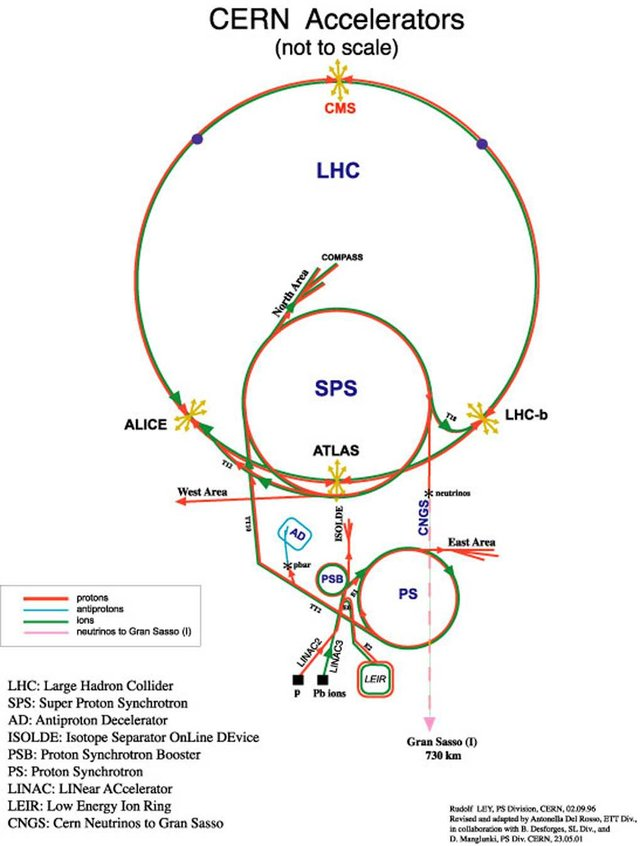
\includegraphics[width=0.9\linewidth]{figures/lhc/injection.jpg}
    \caption{ CERN accelerator complex} 
    \label{fig:injection_chain} 
  \end{center} 
\end{figure}

We begin with the most common element in the Universe, hydrogen, as our source
of protons.  A bottle of hydrogen gas provides 100 microsecond pulses of raw
$H_{2}$ which is then injected into a Duoplasmatron. There,  a strong electric
field and free elctrons from a cathode ionize the molecule into bare $H^{+}$ aka
a proton!  These protons are then accelerated by a 90kV field, leaving the
Duoplasmatron with 1.4\% speed of light ($\sim$4000km/s) or, in relativistic
units, about 83keV. The bare protons are then fed into the accelerating
RadioFrequency (RF) cavities of Linear Accelerator 2 (LINAC2). Inside,
conductors charged by a powerful oscillating electromagnetic field accelerate
the protons resulting in a 50MeV energy. Along the way, small quadrupole magnets
shape the proton packet insuring they remain in a tight beam.  This pattern of
accleration with RF cavities and shaping/turnig with magnets is then repeated
with CERN's first synchrotron, the Proton Synchrotron (PS) rendering a 1.4 GeV
beam.  The final step before the LHC comes with the Super Proton Synchrotron
where the same technologies are implemented to produce 450 GeV protons, ready
for injection into the LHC. A diagramatic representation of this chain can be
seen in figure \cite{injection_chain} 

In order to produce proton-proton collisions the LHC uses two beams circulating
in opposite directions.  The beams are not continuous, but instead consist of
bunches, or buckets, of $\mathcal{O}(10^{11})$ protons with a spacing of 25ns.
Given the LHC circumference this allows for 3564 buckets, however only 2808 are
filled per beam due to safety requirements and injection limitations.  Each beam
takes 4 minutes and 20 seconds to fill and then an additional 20 minutes to for
the protons to reach their maximum energy of 7 TeV TeV, or 99.99999991\% the
speed of light! Under normal operating conditions these beams can be used for
many hours.

\section{Accelerator complex layout and design} \label{sec:lhc:layout}

We begin with the most common element in the Universe, hydrogen, as our source
of protons.  A bottle of hydrogen gas provides raw $H_{2}$ which is then
injected into a Duoplasmatron which uses a strong electric field to break the
molecule into bare $H^{+}$ aka a proton!  The proton is then accelerated by a 90
kV supply and leaves the Duoplasmatron with 1.4\% speed of light (~4000
km/s).


\section{Performance} \label{sec:lhc:performance}

Since the begining of its stable running in 2010 the LHC has performed well,
even exceeding our expectations.  While the experiment itself is incredibly
complex, the performance of the machine, for the purposes of our analysis, can
be reduced to two numbers; the familiar center of mass energy of the beams and a
less common quantity known as the integrated luminosity.  

For particle physics the integrated luminosity is proportional to the total
number of collisions recorded during a specified time period, while the
instantaneous luminosity is proportional to the bunch crossing rate along with
the cross section of a proton-proton interaction and represents the potential
number of collisions per second.  Knowing this we can see that the integrated
luminosity, $L_{int}$ is simply the integral of the instantaneous luminosity
$L_{inst.}$ for a choosen data period as seen in equation XXX.

$$ L_{int} = \int L_{inst.}dt $$

For a standard Gaussian beam, $L_{inst.}$ can be written as

$$ L = \frac{N_{b}^{2}n_{b}f_{rev}\gamma_{r}}{4\pi\epsilon_{n}\beta^{*}}F $$,

where $N_{b}$ is the number of particles per bunch, $n_{b}$ the number of
bunches per beam, $f_{rev}$ the revolution frequency, $\gamma_{r}$ the
relativistic gamma factor, $\epsilon_{n}$ the normalized transverse beam
emittance, $\beta^{*}$ the beta function at the collision point, and $F$ the
geometric luminosity reduction factor due to the crossing angle at the
interaction point given by

$$ F = \bigg(1 + \Big( \frac{\theta_{c}\sigma_{z}}{2\sigma^{*}} \Big) ^{2}
\bigg)^{-1/2} $$,

where $\theta_{c}$ is the full crossing angle at the interaction point,
$\sigma_{z}$ is the RMS bunch length, and $\sigma^{*}$ is the transverse RMS
beam size at the interaction point.

For the ATLAS experiment the integrated luminosity for each year can be seen in
figure XXX as well as an example of the instantaneous luminosity for the choosen
year in figure XXX.

\section{Pile-up at the LHC} \label{sec:lhc:pileup}

Given the large number of protons per bunch and the cross-section of a
proton-proton interaction, the probability to observe multiple interactions per
bunch crossing is quite high.  These multiple-interaction are known as pile-up,
$\mu$ or the time averaged representation $\langle \mu \rangle$, and come in two
different forms: 

\begin{enumerate} \item \textbf{In-time pile-up:} These are the other
proton-proton collisions that occur during the same bunch crossing as the
primary interaction that cauesd the Data Aquisition (DAQ) system to trigger.
These are the standard extra interactions we expect to observe as stated above.
\item \textbf{Out-of-time pile-up:} These are interactions that occur either
before or after a bunch crossing that causes the DAQ to trigger.  This effect is
generally due to the long integration times of some detector electronics.
\end{enumerate}

The pile-up profile for past years can be seen in figure XXX.  The width of this
distributino is due a combination of Poisonian statistics, the decrease in
number of protons per bunch over the lifetime of a single run, and optimization
tweaks to the beam's profile during runtime.  Understanding and eliminating the
noise from these pile-up events is crucial to reconstructing physics variables
to represent the primary interaction we hope to observe.

